\section{Chandra Kirana Poetra (1174079)}
\subsection{Buku}
Rp.100.000(Lunas)
\subsection{Data Geospasial}
\begin{itemize}
	\item Data Geospasial merupakan informasi lokasi geografis, dimensi, ukuran, atau karakteristik objek alam yang berada pada permukaan 	bumi yang disimpan pada sistem informasi geografis, 
	\item Tipe dari data geografis
	\begin{enumerate}
\begin{figure}[H]
	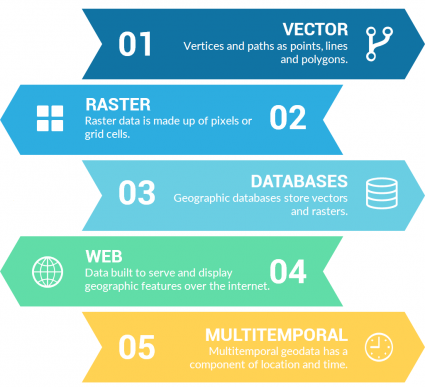
\includegraphics[width=8cm]{figures/Tugas1/1174079/vector.png}
	\centering
	\caption{Tipe data Geospasial.}
\end{figure}	

	\item Vector merupakan tipe data yang mencakup vertices dan juga path. 3 hal mendasar dari sebuat vector merupakan point, garis, dan juga polgyons. setiap point, garus dan polygon mempunyai referensi spasial seperti latitude dan longitude. Point vector berisi koordinat X dan Y, kemudian lines akan menghubungkan kedua point atau bisa juga disebut sebagai vertex, selanjutnya polgons akan menggabungkan semua vertices.
	
	\item Data Raster terbuat dari piksel dan juga cell grid. raster kebanyakan berbentuk kotak, atau bisa juga kubus. Raster akan memberikan nilai kesetiap pixes yang ada, Continuous raster mempunyai nilai yang akan selalu berubah seperti ketinggian dan temperatur. tetapi diskrit raster membuat setiap piksel menjadi class yang spesifik.
	\item Geografik Databases memiliki tujuan untuk menyimpan vector dan juga rasters. database menyimpan data geografik sebagai suatu data atau informasi yang terstruktur. Kita menggunakan database geografik karena database ini mempermudah penarikan data menjadi satu bungkusan atau package sehingga menjadi lebih mudah untuk membuat versi tersendiri ataupun hal-hal lain.
	\item Web Files seperti GeoJSON , GeoRSS dan web mapping services digunakan untuk melayani dan memperlihatkan data geografis melalui internet.
	\item Multitemporal Data menyisipkan komponen waktu ke suatu informasi geografis seperti contohnya data cuaca dan musim yang perlu di monitor temperatur dan juga informasi meteorologinya yang selalu berubah seiring dengan berjalannya waktu


	\end{enumerate}
\end{itemize}

\subsection{Link}
https://youtu.be/vzRFyiYVAUY
\subsection{Plagiarism}'\begin{figure}[H]
	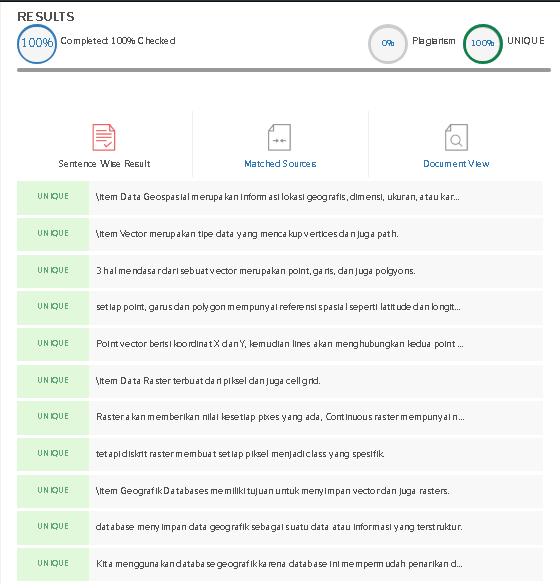
\includegraphics[width=8cm]{figures/Tugas1/1174079/plagiarisme.png}
	\centering
	\caption{Plagiarisme.}
\end{figure}	

\subsection{Cara Penggunaan}
\subsubsection{Gambar}

\hfill\break

Contoh Gambar
\begin{figure}[H]
	
\includegraphics[width=4cm]{figures/himatif.png}
	\centering
	\caption{Contoh gambar.}
\end{figure}

\subsubsection{List}
\begin{enumerate}
	\item Satu
	\item Dua
\end{enumerate}

\begin{itemize}
	\item Satu
	\item Dua
\end{itemize}

